% ---------- in your preamble ----------
\usetikzlibrary{positioning}
% --------------------------------------

\begin{figure}[t]
  \centering
  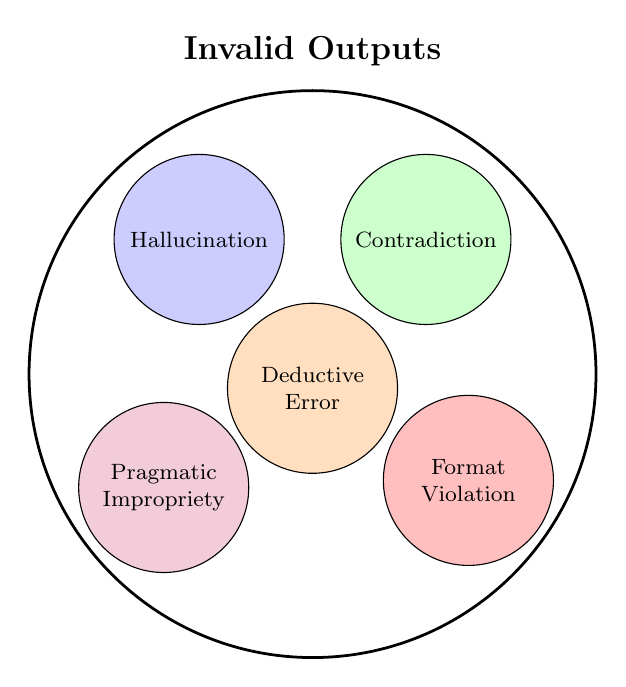
\begin{tikzpicture}[scale=0.9]

    % --- outer (universal) set ---
    \draw[line width=1pt] (0,0) circle (4cm);
    \node[font=\large\bfseries] at (0,4.55) {Invalid Outputs};

    % --- subclasses ---
    \begin{scope}[every node/.style={font=\footnotesize,align=center}] % <-- align added
      % Hallucination
      \filldraw[fill=blue!20,draw=black] (-1.6,1.9) circle (1.2cm);
      \node at (-1.6,1.9) {Hallucination};

      % Contradiction
      \filldraw[fill=green!20,draw=black] (1.6,1.9) circle (1.2cm);
      \node at (1.6,1.9) {Contradiction};

      % Deductive error
      \filldraw[fill=orange!25,draw=black] (0,-0.2) circle (1.2cm);
      \node at (0,-0.2) {Deductive\\Error};

      % Pragmatic impropriety
      \filldraw[fill=purple!20,draw=black] (-2.1,-1.6) circle (1.2cm);
      \node at (-2.1,-1.6) {Pragmatic\\Impropriety};

      % Format violation
      \filldraw[fill=red!25,draw=black] (2.2,-1.5) circle (1.2cm);
      \node at (2.2,-1.5) {Format\\Violation};
    \end{scope}

  \end{tikzpicture}
  \caption{Venn-style illustration of members of a broader set of invalid outputs produced by large language models.}
  \label{fig:taxonomy}
\end{figure}
